\documentclass[%
	paper=A4,	% stellt auf A4-Papier
	pagesize,	% gibt Papiergröße weiter
	DIV=calc,	% errechnet Satzspiegel
	smallheadings,	% kleinere Überschriften
	ngerman		% neue Rechtschreibung
]{scrartcl}
\usepackage{BenMathTemplate}
\usepackage{BenTextTemplate}

\title{{\bf Wissenschaftliches Rechnen III / CP III}\\Übungsblatt 4}
\author{Tizia Kaplan (545978)\\Benjamin Dummer (532716)\\ Gruppe 10}
\date{25.05.2016}

\begin{document}
\maketitle
Online-Version: \href{https://www.github.com/BeDummer/CP3_UE4}{\url{https://www.github.com/BeDummer/CP3_UE4}}

\section*{Aufgabe 4.i}

\begin{figure}[!b]
  \centering
  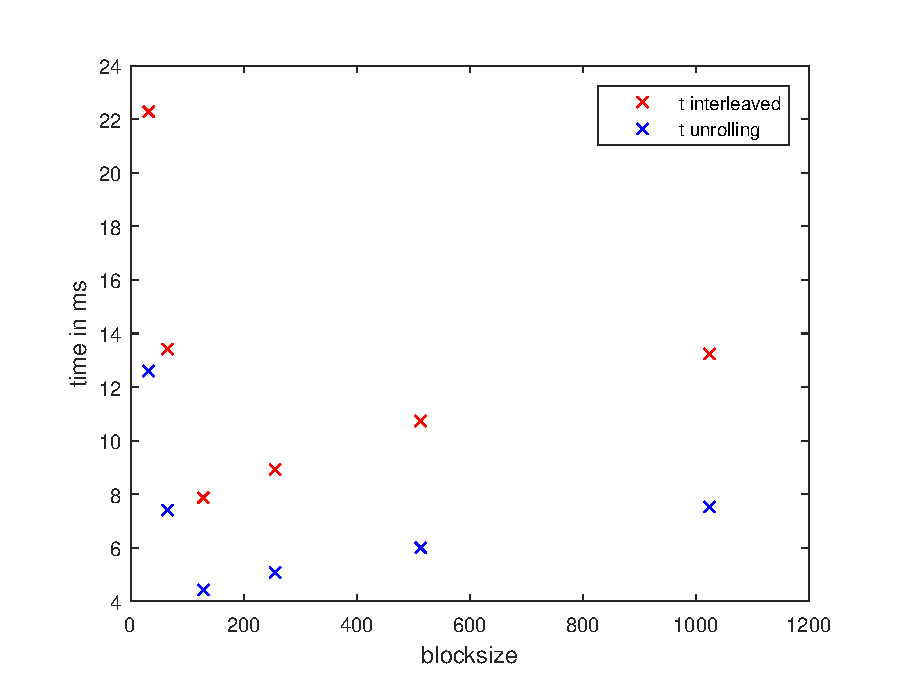
\includegraphics[width=.75\textwidth]{blocksize_vs_time_interl_unroll.eps}
  \caption{Blocksize vs. Simulationszeit f"ur die unterschiedlichen Realisierungen der parallelen Reduktion (interleaved \& unroll)}
\end{figure}

Hier sollten die Laufzeiten f"ur $n=2^{24}$ Elemente f"ur unterschiedliche Blockgr"o\ss en mithilfe von \texttt{nvprof ./a.out} gemessen werden. Vergleichend wurden die Simulationszeiten f"ur die Implementierungen \texttt{reduceInterleaved} und \texttt{reducedUnrolling} aufgenommen. Gefunden wurde ein Minimum bei der Blockgr"o\ss e $128$ (siehe Abb. 1) 

\section*{Aufgabe 4.ii}
Nun konnten auch Global Memory Load Efficiency, Global Load Throughput und Achieved Occupancy gemessen werden. Hier wurden mittels \url{nvprof --metrics gld_efficiency,gld_throughput,achieved_occupancy ./a.out} die Durchschnittswerte ermittelt. Die Ergebnisse sind in den Abb. 2 bis 4 gezeigt.

\begin{figure}[!hb]
  \centering
  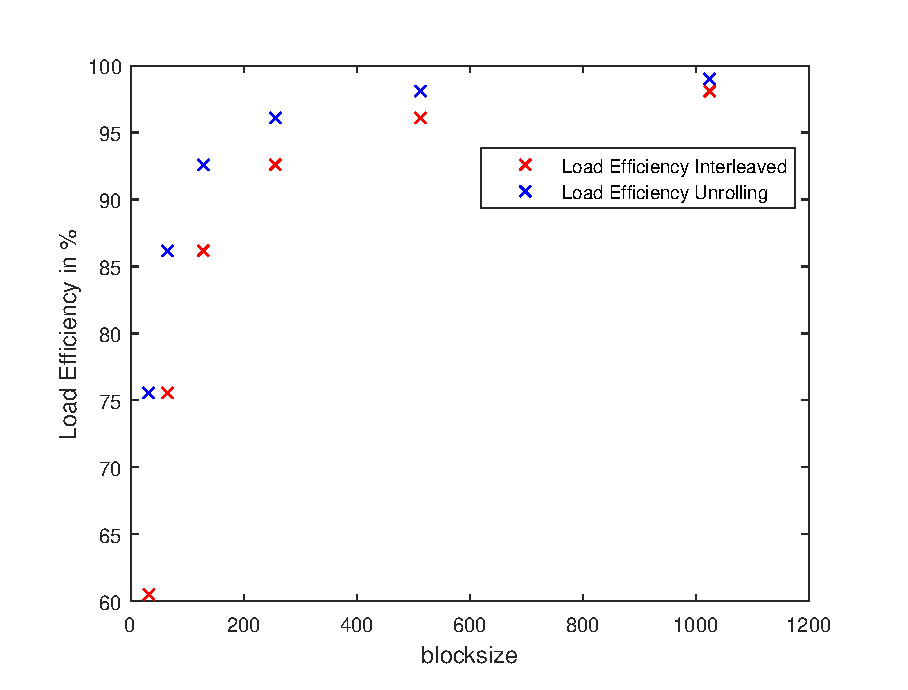
\includegraphics[width=.75\textwidth]{blocksize_vs_load_efficiency.eps}
  \caption{Blocksize vs. Global Memory Load Efficiency f"ur die unterschiedlichen Realisierungen der parallelen Reduktion (interleaved \& unroll)}

  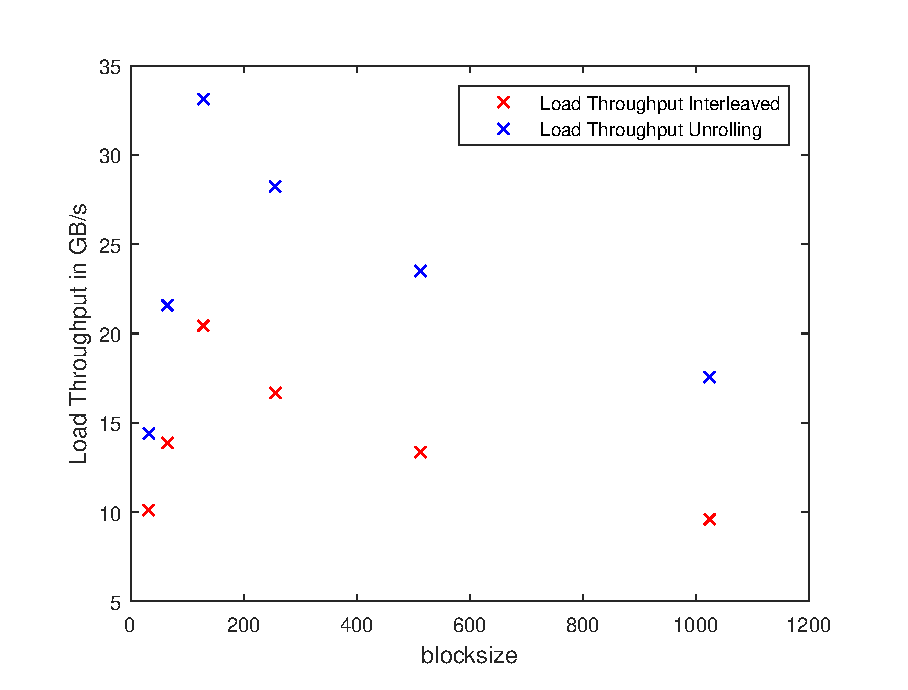
\includegraphics[width=.75\textwidth]{blocksize_vs_load_throughput.eps}
  \caption{Blocksize vs. Global Load Throughput (Bandbreite) f"ur die unterschiedlichen Realisierungen der parallelen Reduktion (interleaved \& unroll)}
\end{figure}
\begin{figure}
  \centering
  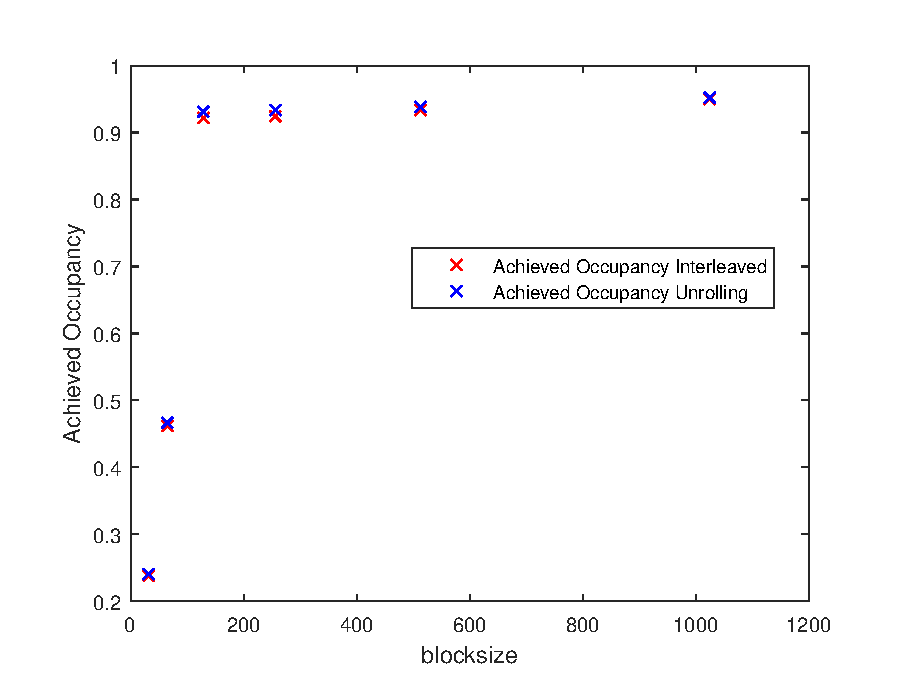
\includegraphics[width=.75\textwidth]{blocksize_vs_achieved_occ.eps}
  \caption{Blocksize vs. Achieved Occupancy f"ur die unterschiedlichen Realisierungen der parallelen Reduktion (interleaved \& unroll)}
\end{figure}

\section*{Aufgabe 4.iii}
Man erkennt eine Laufzeitverbesserung f"ur Blockgr"o\ss en bis $128$ und diese erreicht dort ein Minimum. Die Verbesserung wird auch deutlich durch steigende Werte der in ii) gemessenen Parameter. Ab der Blockgr"o\ss e $128$ jedoch, "andern sich die \emph{Load Efficiency} und die \emph{Achieved Occupancy} nur unwesentlich - die Bandbreite sinkt jedoch wieder ab. Dementsprechend gibt es ein Minimum der Laufzeit bei Blockgr"o\ss e $128$.

In Abb. 1 l"asst sich au\ss erdem noch eine starke Differenz der Laufzeiten zwischen \emph{Interleaved} und \emph{Unrolling} erkennen. Unter einer Blockgr"o\ss e von $128$ ist die \emph{Load Efficiency} ausschlaggebend f"ur die Laufzeitunterschiede. Danach nimmt die Bandbreite den entscheidenden Einfluss auf die Differenz.

Eine Idee zur Erkl"arung des Minimums bei einer Blockgr"o\ss e von $128$ ist die Anzahl der Kerne pro \emph{Streaming Multiprocessor}. Diese liegt bei $192$. Wenn ein Thread-Block nun gr"o\ss er als $192$ ist, k"onnen nicht mehr alle Operationen pro Block gleichzeitig ausgef"uhrt werden und das System muss warten.

\section*{Aufgabe 4.iv}
Hier wurde $q$ als Potenz von $2$ implementiert. Das Optimum der Laufzeit wurde f"ur  alle Blockgr"o\ss en (analog zu i) ) im Bereich $1024=2^{10}\leq q \leq 2^{11}=2048$ gefunden. Auffallend war, dass $q$ einen Einfluss auf die absolute Laufzeit der unterschiedlichen Blockgr"o\ss en hatte: im Test wurde die schnellste Laufzeit von $t_{unrollOpt}=1.42 ms$ f"ur eine Blockgr"o\ss e von $1024$ gefunden, allerdings variieren die Laufzeiten ab einer Blockgr"o\ss e von $128$ nur im Bereich von $10-20 \mu s$.

Warum gilt das Laufzeitminimum f"ur eine Blockgr"o\ss e von $128$ hier nicht?\\
Dadurch, dass mehrere Operationen pro Kern durchgef"uhrt werden, wird die Bandbreite optimal ausgesch"opft und der Einfluss des \glqq Wartens \grqq verschwindet.

\section*{Aufgabe 4.v}
Ausgehend von unserer Analyse in iv) haben wir nun unsere optimierte Reduktion f"ur den Datentyp \texttt{double} mit den optimalen Parametern (Blockgr"o\ss e $1024$ und $q=2048$) erweitert. Der Vergleich zwischen den beiden Implementierungen (\texttt{int} vs. \texttt{double}) liefert folgende Ergebnisse:

\begin{eqnarray} \nonumber
	\begin{array}{l|c|c}
 \mbox{Variablentyp} & \mbox{\tt int} & \mbox{\tt double}\\ \hline
 \mbox{Laufzeit [ms]} & 1.47 & 2.01  \\ 
 \mbox{Efficiency [\%]} & 100 & 100 \\
 \mbox{Throughput [GB/s]} & 47.8 & 69.4  \\
 \mbox{Occupancy} & 0.9985 & 0.9992
	\end{array}
\end{eqnarray}

Der Datentyp \texttt{double} hat einen h"oheren Speicherbedarf, dadurch kann die Bandbreite noch besser ausgenutzt werden. Da diese allerdings nach oben begrenzt ist, verl"angert sich die Simulationszeit.

\section*{Anhänge}
\begin{itemize}
	\item Datei: \url{reduction_w_q.cu} (Suche nach optimalem $q$)
	\item Datei: \url{reduction_w_q_fix.cu} (\texttt{int}-Implementierung f"ur Vergleich mit \texttt{double}-Implementierung)
	\item Datei: \url{reduction_double.cu} (\texttt{double}-Implementierung mit optimierten Parametern)
\end{itemize}
\end{document}
